\section{Visualization}\label{sec:visualization}
The following visualizations each address a distinct question about the Citi Bike system. This section presents them in turn, detailing the specific encodings, supported interactions, and underlying design decisions involved.
Before covering each view individually, the following two subsections introduce the shared technical implementation and consistent design language behind them.

\begin{figure}[htbp]
    \centering
    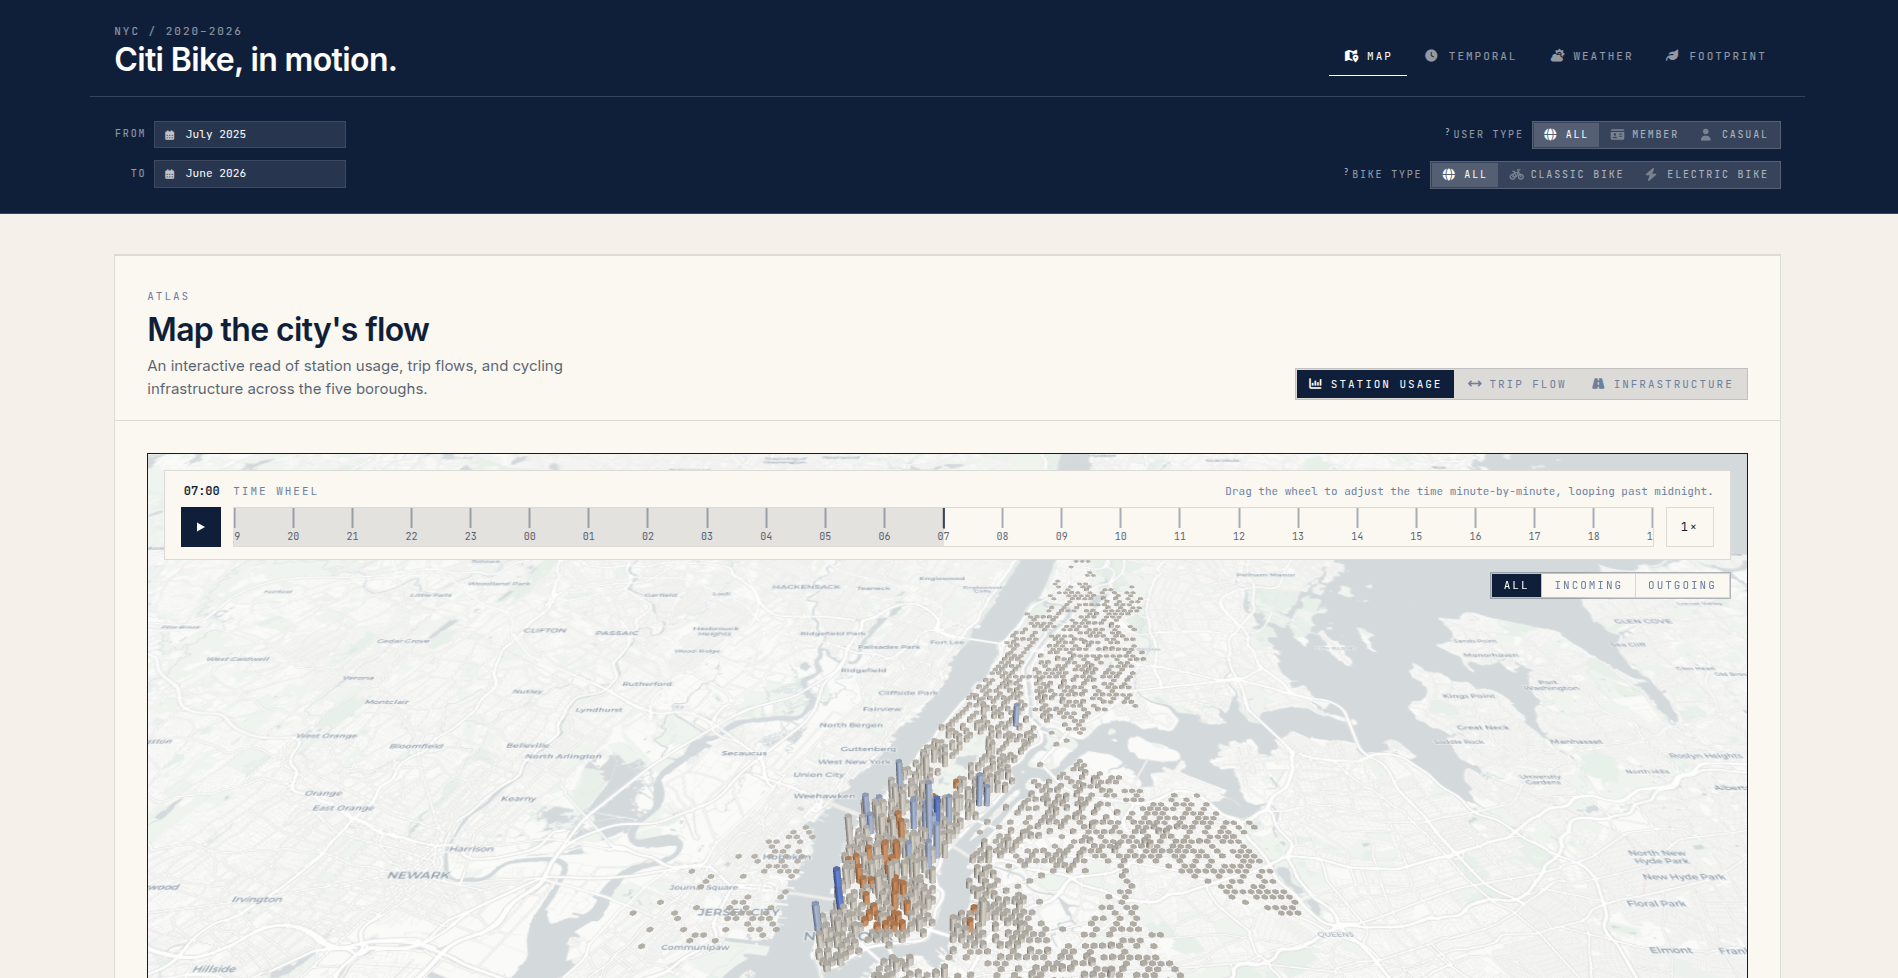
\includegraphics[width=\textwidth]{../media/report/starting_page.png}
    \caption{Dashboard: the starting view.}
    \label{fig:viz-overview}
\end{figure}

\subsection{Implementation}
The frontend is a \emph{React} application built with \emph{Vite} and routed via \emph{React Router}.
Layout and visual design tokens are managed through a unified \emph{Tailwind CSS} module, ensuring consistent styling across interface components, charts, and maps.

Each view employs a library tailored to its specific data structures:
\begin{itemize}
    \item \textbf{deck.gl} renders \emph{WebGL} map layers, maintaining interactive performance across thousands of stations and arcs.
    \item \textbf{Plotly} generates three-dimensional surfaces and distribution plots.
    \item \textbf{Chart.js} and custom canvas to draw simple 2D charts.
\end{itemize}

Although the original proposal specified \emph{D3.js} for non-map charts,
using \emph{Plotly} and \emph{Chart.js} for standard visuals saved development time.
\emph{D3.js} provides no ready-made charts, so every axis, scale, and update animation has to be written by hand.
Both libraries animate data changes on their own, and a single duration and easing setting keeps motion consistent across every chart.

\subsection{User Experience}
To maintain consistency, all components share a standardized layout skeleton: a descriptive header, a primary display, secondary plots, and a collapsible reading guide.
Notably, these secondary plots expand upon the initial proposal by providing additional context around the core insights.

\paragraph{Visual Design}
To prioritize data clarity over decorative clutter, the interface uses a clean design:
\begin{itemize}
    \item \textbf{Color Usage:} Neutral tones for the layout, reserving bright colors strictly to highlight inside charts.
    \item \textbf{Typography:} Clear, readable fonts applied consistently across all views.
    \item \textbf{Animation:} Minimal motion to enhance the user experience without adding distraction.
\end{itemize}

\paragraph{Interaction Model}
Because the dashboard is exploratory, ensuring immediate clarity without enforcing a narrative was a primary design concern.
We adopted a three-part interaction model:
\begin{itemize}
    \item \textbf{Guide:} Each view has a collapsible ``How To Read It'' panel (Figure~\ref{fig:viz-guide}) with three practical hints, giving users a clear starting point for exploration.
    \item \textbf{Tooltips:} Embedded hints and hover-triggered tooltips surface exact values and fine-grained details on demand, permitting to have a complete overview without overwhelming.
    \item \textbf{Defaults:} Sensible default states offer immediate global insights, while interactive filters, toggles, and linked selections enable deeper inspection on demand.
\end{itemize}

\begin{figure}[htbp]
    \centering
    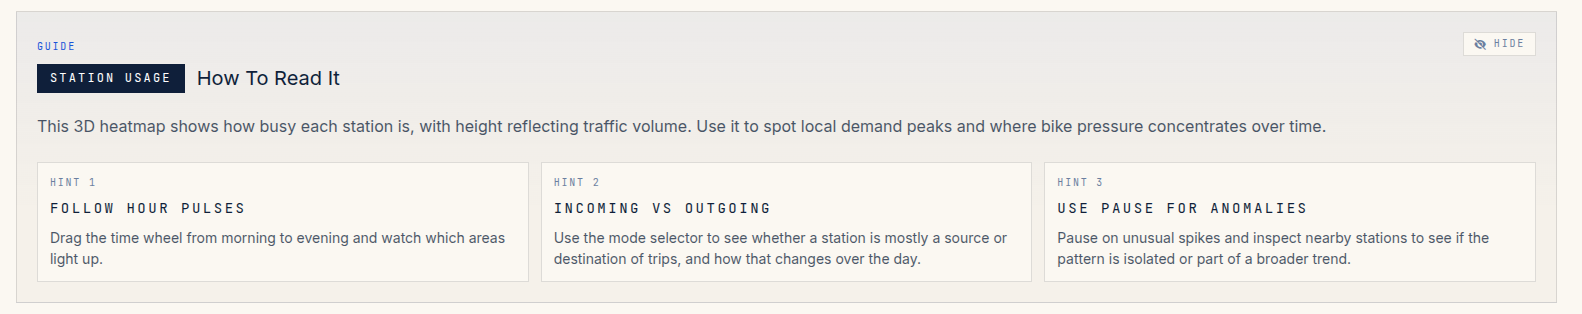
\includegraphics[width=\textwidth]{../media/report/guide.png}
    \caption{Dashboard: the reading guide.}
    \label{fig:viz-guide}
\end{figure}

\subsection{Header}
The global header incorporates two primary filter controls (Figure~\ref{fig:viz-filters}):
\begin{itemize}
    \item \textbf{Date Range Picker:} A monthly calendar selector with a $12$-month maximum range.
    Maximum ranges too short would limit trend visibility, while ranges too long would slow down performance.
    \item \textbf{User and Bike Type Selectors:} A pair of selectors filtering data by membership status (member or casual) and bike type (classic, electric, or both).
\end{itemize}
Changing any global filter automatically reloads the charts while keeping selections active across pages.
The precomputation described in Section~\ref{sec:data-pipeline} keeps these reloads fast.

\paragraph{Response Caching}
Beyond how fast each query resolves, performance also depends on how often the same request repeats.
Our dashboard requires multiple queries across multiple pages and filters, which can lead to repeated requests for the same data.
The frontend caches (\emph{TanStack Query}) responses keyed by their exact filter set, allowing revisited views to render instantly.

\paragraph{Cross-filtering}
These global filters narrowed the cross-filtering planned in our proposal.
To address this, we added view-specific filters that operate independently of the header.
Additionally, filters that were only relevant to specific views were removed from the global header and relocated.

\begin{figure}[htbp]
    \centering
    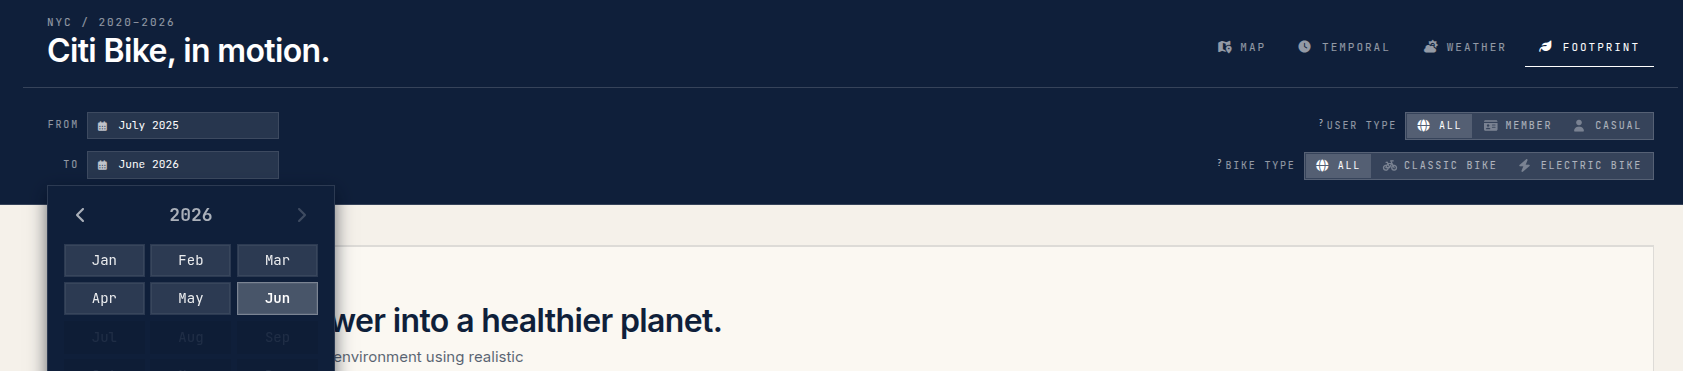
\includegraphics[width=\textwidth]{../media/report/header.png}
    \caption{Dashboard: the global header.}
    \label{fig:viz-filters}
\end{figure}

\subsection{Map}
As the dashboard's default view (Figure~\ref{fig:viz-overview}), the spatial map offers an immediate, impactful geographic overview.
Multiple relevant spatial insights can be extracted from the Citi Bike dataset, including station usage, trip flow, and infrastructure.
We chose to break down the analysis into three focused map layers rather than combining them into one view.

\subsubsection{Station Usage}
This layer establishes where demand concentrates across the network, summarizing station activity into a form that remains clear at city scale.

\paragraph{Hexagon Heatmap}
By aggregating individual stations into hourly bins, we visualize the overall activity distribution across space and time of day.
Figure~\ref{fig:viz-station-usage} presents a 3D heatmap of elevated hexagons, where height encodes absolute usage and color highlights deviation from mean activity.
This dual encoding makes it easy to spot spatial anomalies in both absolute and relative terms.

Other visualizations were considered, including choropleth maps and 2D heatmaps.
However, displaying thousands of stations and millions of rides often led to overcrowded, unreadable views.
For instance, a 2D heatmap resulted in heavy overlap, turning the whole city red without any specific zoom.
In contrast, our 3D encoding overcomes this issue by using multiple visual channels.

\paragraph{Map Controls}
While effective for overall spatial trends, the 3D hexagon heatmap alone abstracts away time and other key filters.
To restore this depth, the layer uses precomputed hourly trip counts (Section~\ref{sec:data-pipeline}) and includes a mode selector to isolate incoming, outgoing, or total trips.
This reveals both heavy-traffic stations and top destinations.

Temporal navigation is managed through an interactive time wheel with play controls to animate daily average usage.
Because the hourly raw data created an inconsistent transition, the time wheel linearly interpolates between adjacent hourly averages.
This design trade-off provides a continuous, fluid animation at the expense of showing synthesized intermediate values rather than raw measurements.

\begin{figure}[htbp]
    \centering
    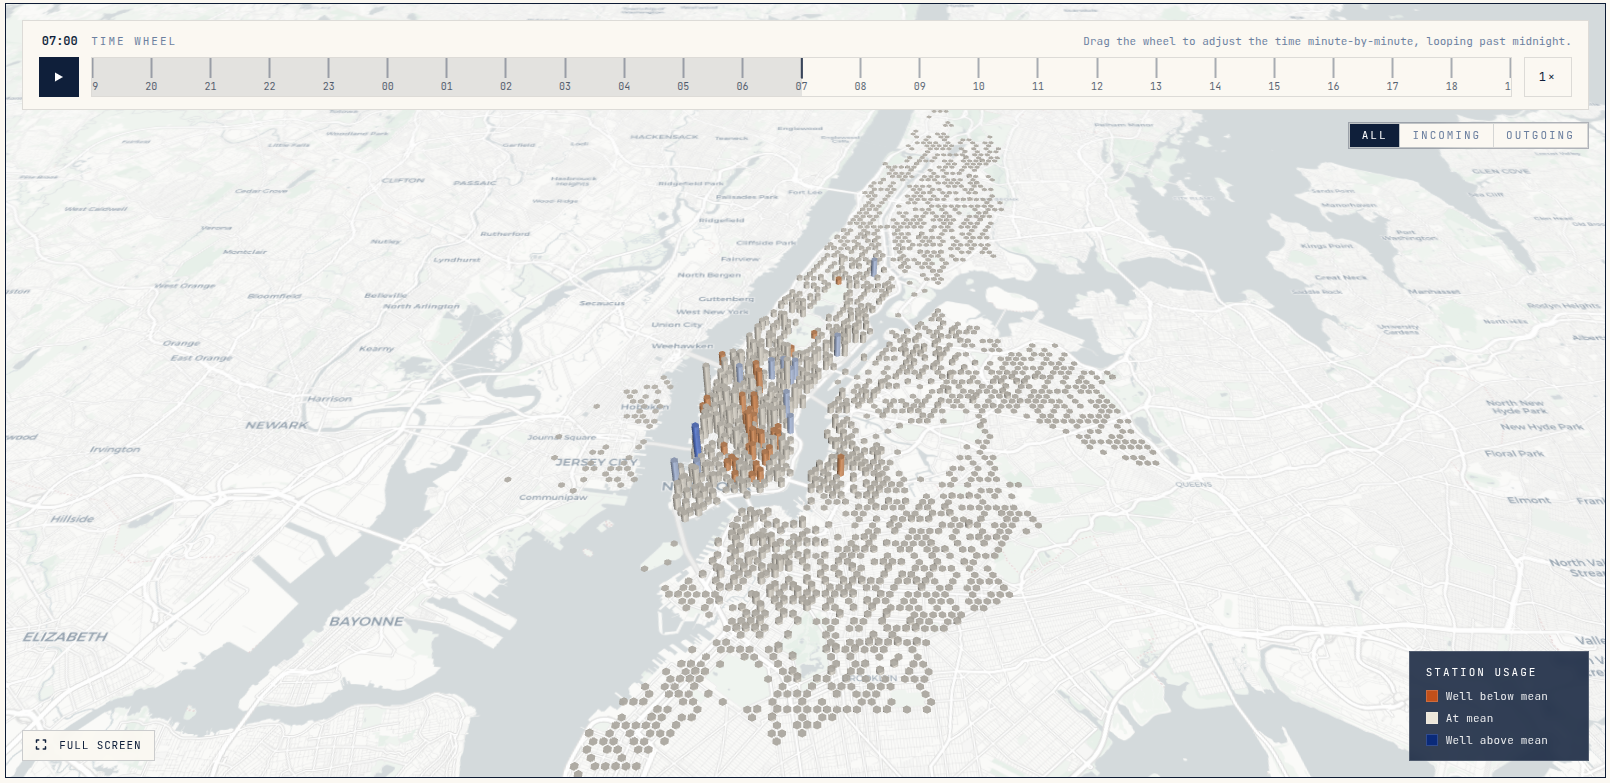
\includegraphics[width=\textwidth]{../media/report/primary_station_usage.png}
    \caption{Station usage: the hexagon heatmap.}
    \label{fig:viz-station-usage}
\end{figure}

\paragraph{Peak Hour and Station Rankings}
To complement the spatial view, two auxiliary plots provide targeted insights (Figure~\ref{fig:viz-secondary-station-usage}):
\begin{itemize}
    \item \textbf{Station Usage by Peak Hour:} A bar chart showing how many stations reach peak activity during each hour of the day. 
    Because selecting a single hour on the 3D map masks city-wide patterns, this view offers an immediate, high-level summary of peak activity distribution across the network.
    \item \textbf{Busiest Stations:} A ranked bar chart highlighting the top stations by average daily trip volume. 
    This eliminates 3D spatial occlusion, allowing users to instantly identify top-performing locations.
\end{itemize}

\begin{figure}[htbp]
    \centering
    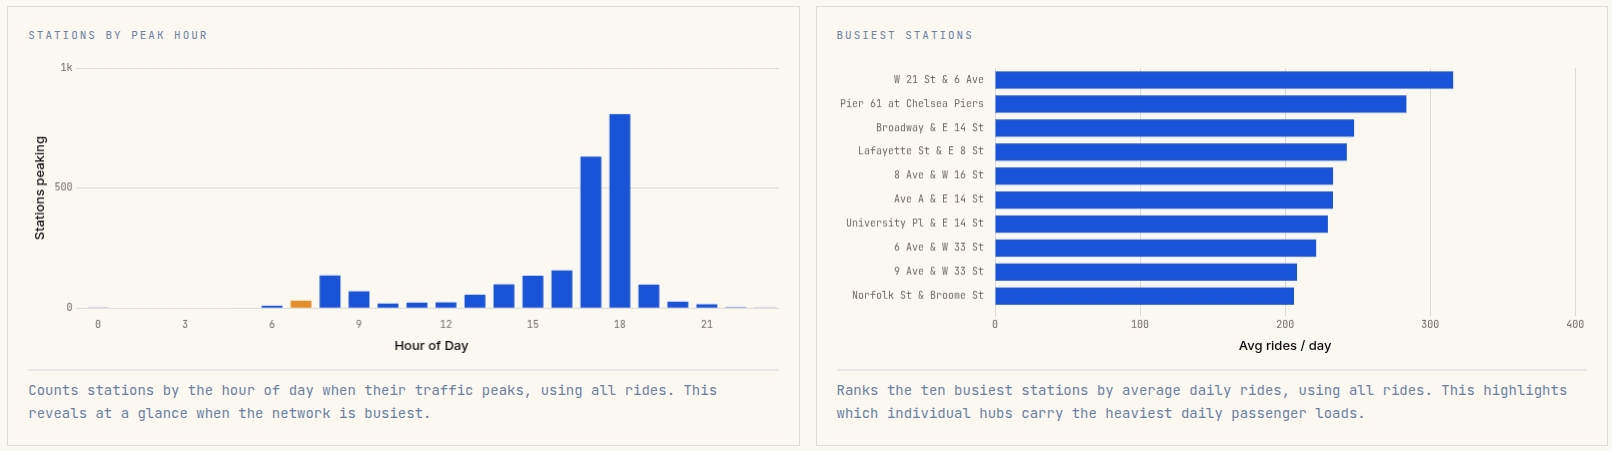
\includegraphics[width=\textwidth]{../media/report/secondary_station_usage.png}
    \caption{Station usage: the supplemental plots.}
    \label{fig:viz-secondary-station-usage}
\end{figure}

\subsubsection{Trip Flow}\label{sec:viz-trip-flow}
While the previous layer quantifies activity at individual stations, this one examines the qualitative connections between them.

\paragraph{Corridor Arcs}
This layer renders origin-destination arcs representing trips between stations, normalized to daily averages for easy comparison across different time periods (Section~\ref{sec:data-pipeline}).
Arc width, together with hue, encodes trip volume, dynamically scaled against the busiest corridor in the current view.
Arc height and curvature carry no quantitative data, as they serve exclusively to disentangle overlapping paths and maintain visual clarity across dense networks.

\paragraph{Citywide Overview}
The initial implementation rendered the entire network simultaneously, producing extreme visual clutter that obscured individual flows.
To resolve this, the second prototype hid all connections by default, revealing top corridors only upon station selection.
While this restored clarity, it completely erased the broader overview and discarded secondary routes.

The final design reconciles both perspectives by rebalancing visual encoding rather than truncating underlying data.
Initial loading presents a citywide overview of the primary transit corridors (Figure~\ref{fig:viz-trip-flow-overview}), providing an immediate macroscopic view of high-volume routes prior to user interaction.

\paragraph{Station Focus}
Selecting an individual station isolates its connected corridors and automatically re-frames the camera view around it (Figure~\ref{fig:viz-trip-flow-single-station}).
Upon selection, color semantics shift from absolute volume to directional flow asymmetry, categorizing links as predominantly inbound, outbound, or balanced.
To avoid misinterpreting minor fluctuations, routes are classified as directional only when traffic strongly favors one side, and as balanced otherwise.

In doing this, we encountered a major data limitation.
Since database rows store station pairs in a canonical order, raw data would randomly assign inbound or outbound labels. 
We resolve this by dynamically reorienting data relative to the selected station. 
\begin{figure}[htbp]
    \centering
    \begin{minipage}[t]{0.49\textwidth}
        \centering
        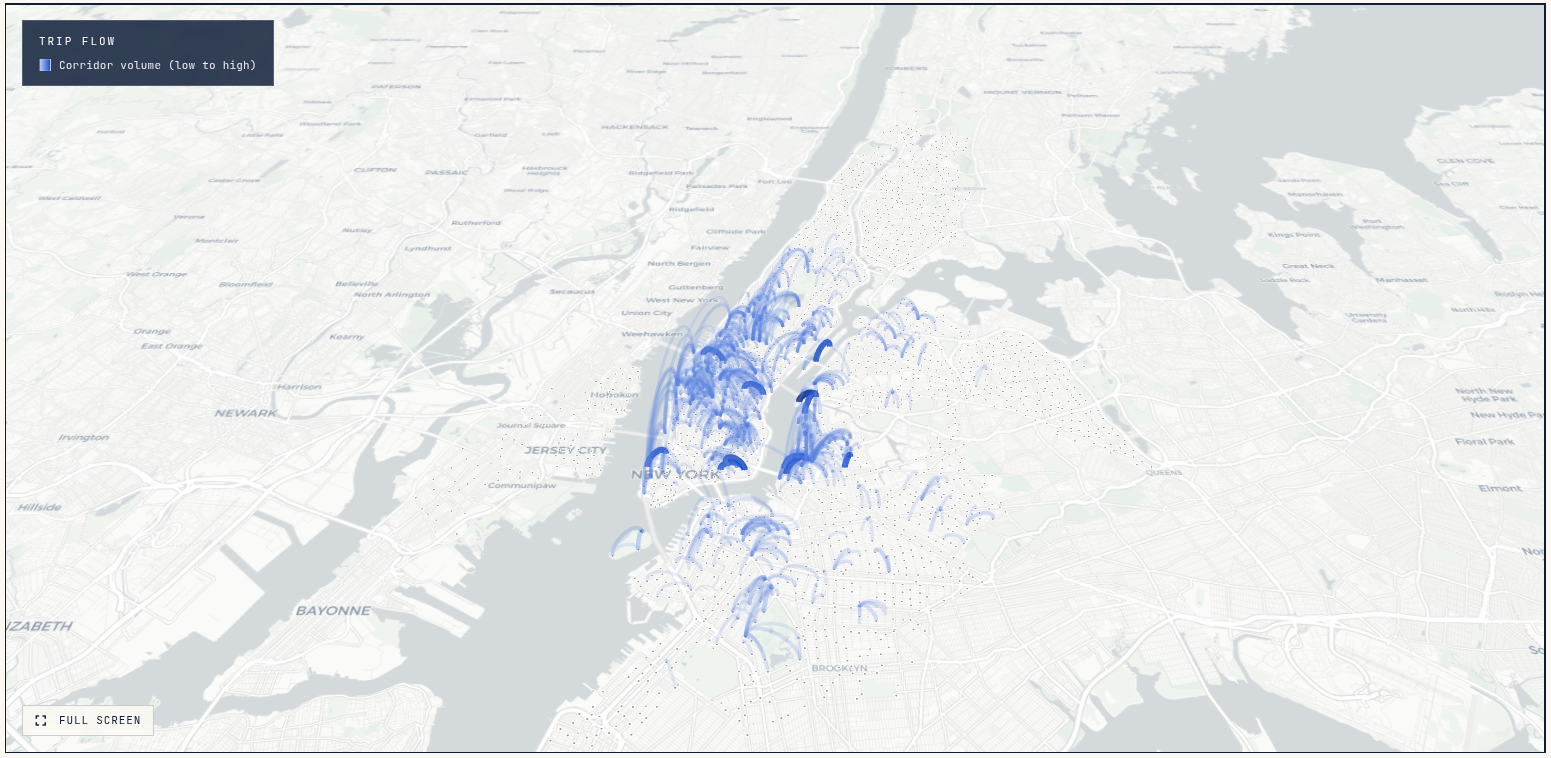
\includegraphics[width=\textwidth]{../media/report/primary_trip_flow_1.png}
        \caption{Trip flow: the citywide overview.}
        \label{fig:viz-trip-flow-overview}
    \end{minipage}
    \hfill
    \begin{minipage}[t]{0.49\textwidth}
        \centering
        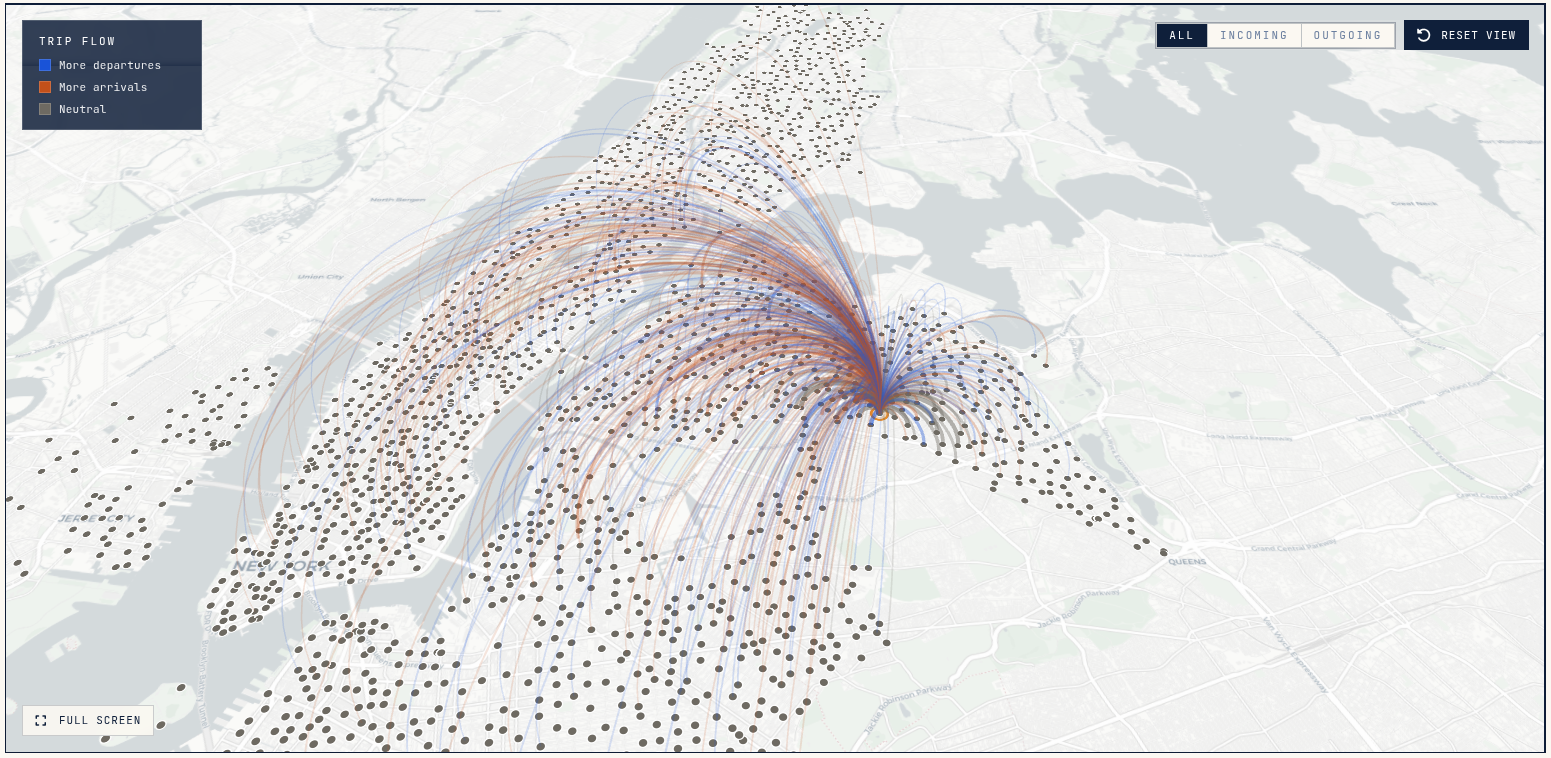
\includegraphics[width=\textwidth]{../media/report/primary_trip_flow_2.png}
        \caption{Trip flow: the station focus.}
        \label{fig:viz-trip-flow-single-station}
    \end{minipage}
\end{figure}

\paragraph{Summary Cards and Corridor Ranking}
Two secondary analytical panels complement the spatial view (Figure~\ref{fig:viz-secondary-trip-flow}):
\begin{itemize}
    \item \textbf{Summary Cards:} Display high-level aggregates for the active context, including total daily rides, active corridor counts, flow-weighted median trip distance, and net directional shares for selected stations.
    This permits users to quickly assess the overall network state without inspecting individual arcs.
    \item \textbf{Ranked Corridor List:} A bar chart illustrating the top twelve corridors of the current selection.
    Interactive hovering highlights the corresponding spatial arc, while clicking a bar isolates that specific corridor by hiding all remaining network links.
    This provides a clear, focused view of the busiest routes.
\end{itemize}

\begin{figure}[htbp]
    \centering
    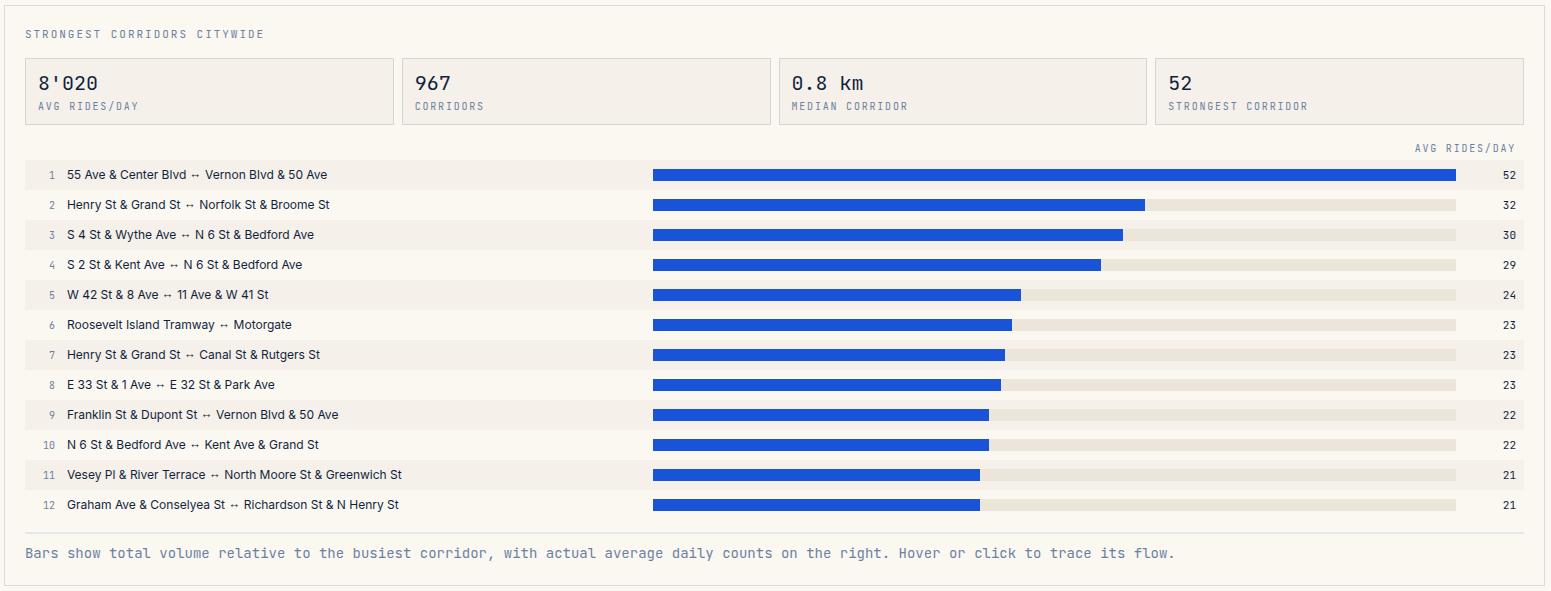
\includegraphics[width=\textwidth]{../media/report/secondary_trip_flow.png}
    \caption{Trip flow: the supplemental plots.}
    \label{fig:viz-secondary-trip-flow}
\end{figure}

\subsubsection{Infrastructure}
Although bike-lane data was excluded from our initial proposal, early analysis showed its value.
Combining lane data with station and route network gave a full picture of the physical infrastructure. 
Additionally, the NYC DOT dataset provided complete, high-quality data, including exact installation and retirement dates for every segment.

\paragraph{Station Status and Bike Routes}
The default view displays real-time station capacity (Figure~\ref{fig:viz-infrastructure}), highlighting nearly empty or full locations so users can spot supply risks at first glance.
Then, by selecting an interactive toggle, users can overlay NYC bike routes (Figure~\ref{fig:viz-infrastructure-bike-routes}).
To prevent visual clutter, we hid the bike routes by default, since segments otherwise would have obscured station locations and their operational status, making them difficult to identify.

\paragraph{Station Sidebar}
Initially, station details were displayed only in hover tooltips.
However, this approach quickly became cluttered and restricted the amount of information we could show.

To provide a comprehensive overview of each station, we introduced a contextual sidebar that opens upon selection, combining real-time and historical metrics (Figure~\ref{fig:viz-station-sidebar}):
\begin{itemize}
    \item \textbf{Live Availability:} Reports effective capacity, open docks, and rentable bikes (disaggregated by classic and electric), alongside out-of-service counts.
    \item \textbf{Historical Profile:} Displays hourly and daily ride distributions, identifying peak usage hours, busiest days, and overall arrival-departure balance.
    \item \textbf{Top Connected Stations:} Ranks the station's five strongest corridors, in order to provide a quick overview of the station's connectivity.
    Selecting a corridor re-centers the interface on the partner station, allowing sequential exploration across connected routes.
\end{itemize}

\paragraph{Year Slider}
A temporal slider completes the infrastructure layer, allowing users to filter bike lanes by installation year.
By rendering only segments active in a selected year, the layer transforms from a static overview into a historical view of NYC's evolving cycling network.

However, this feature introduced a major challenge.
Segments dated \texttt{01/01/1900} predate formal records, so removing them would delete long-standing paths. 
To avoid misleading interpretations, we kept these segments and added a note explaining that this early date represents a historical baseline, not an active construction year.

Moreover, integrating real-time and historical datasets introduced an unavoidable temporal mismatch.
While bike routes include installation and retirement timestamps, station metadata is available only as a live snapshot (Section~\ref{sec:backend}).
Consequently, the temporal slider filters the route network exclusively while holding station locations at their current state, avoiding speculative reconstruction of past station positions.

\begin{figure}[htbp]
    \centering
    \begin{minipage}[t]{0.49\textwidth}
        \centering
        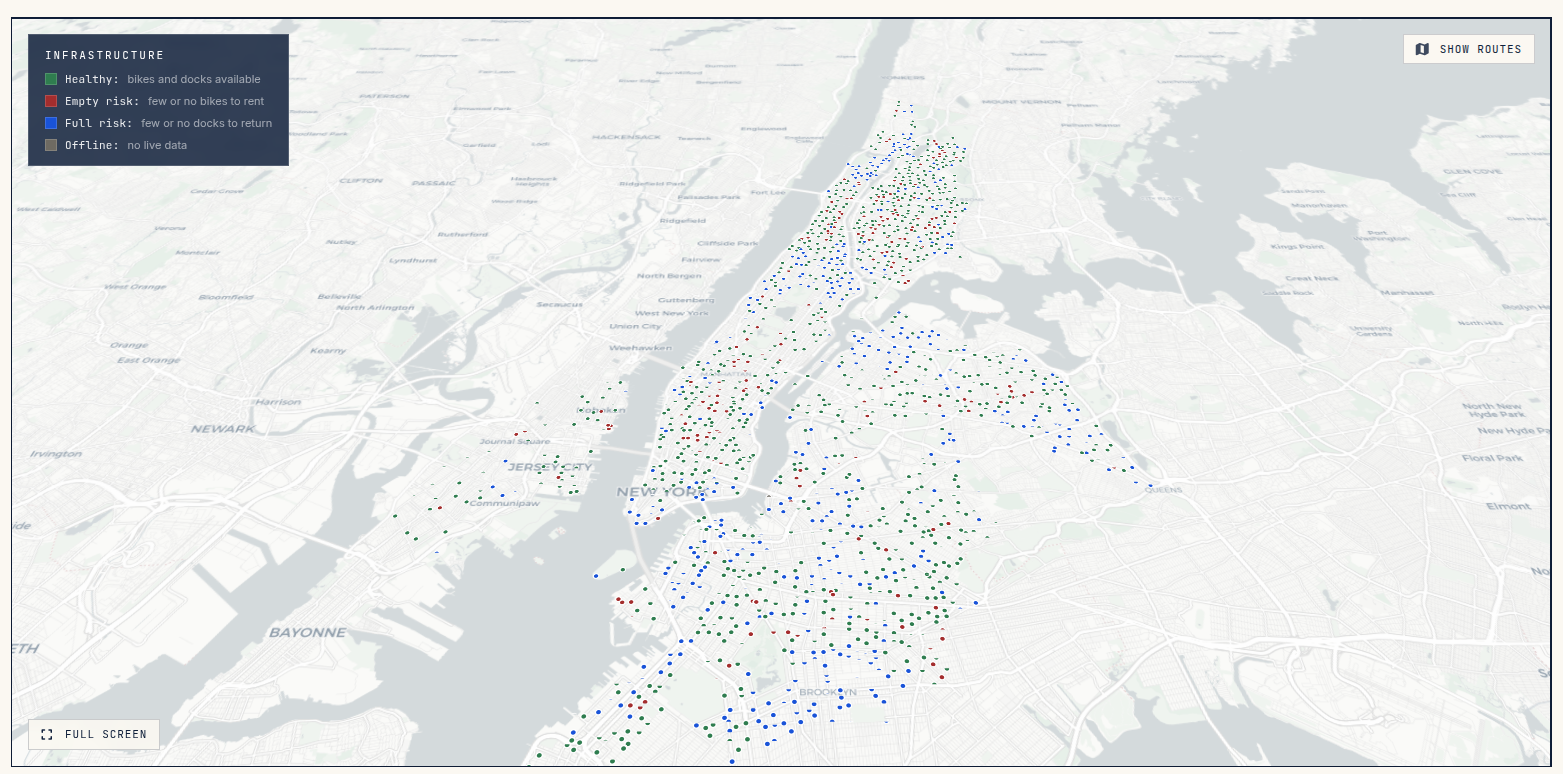
\includegraphics[width=\textwidth]{../media/report/primary_infrastructure_1.png}
        \caption{Infrastructure: the station status.}
        \label{fig:viz-infrastructure}
    \end{minipage}
    \hfill
    \begin{minipage}[t]{0.49\textwidth}
        \centering
        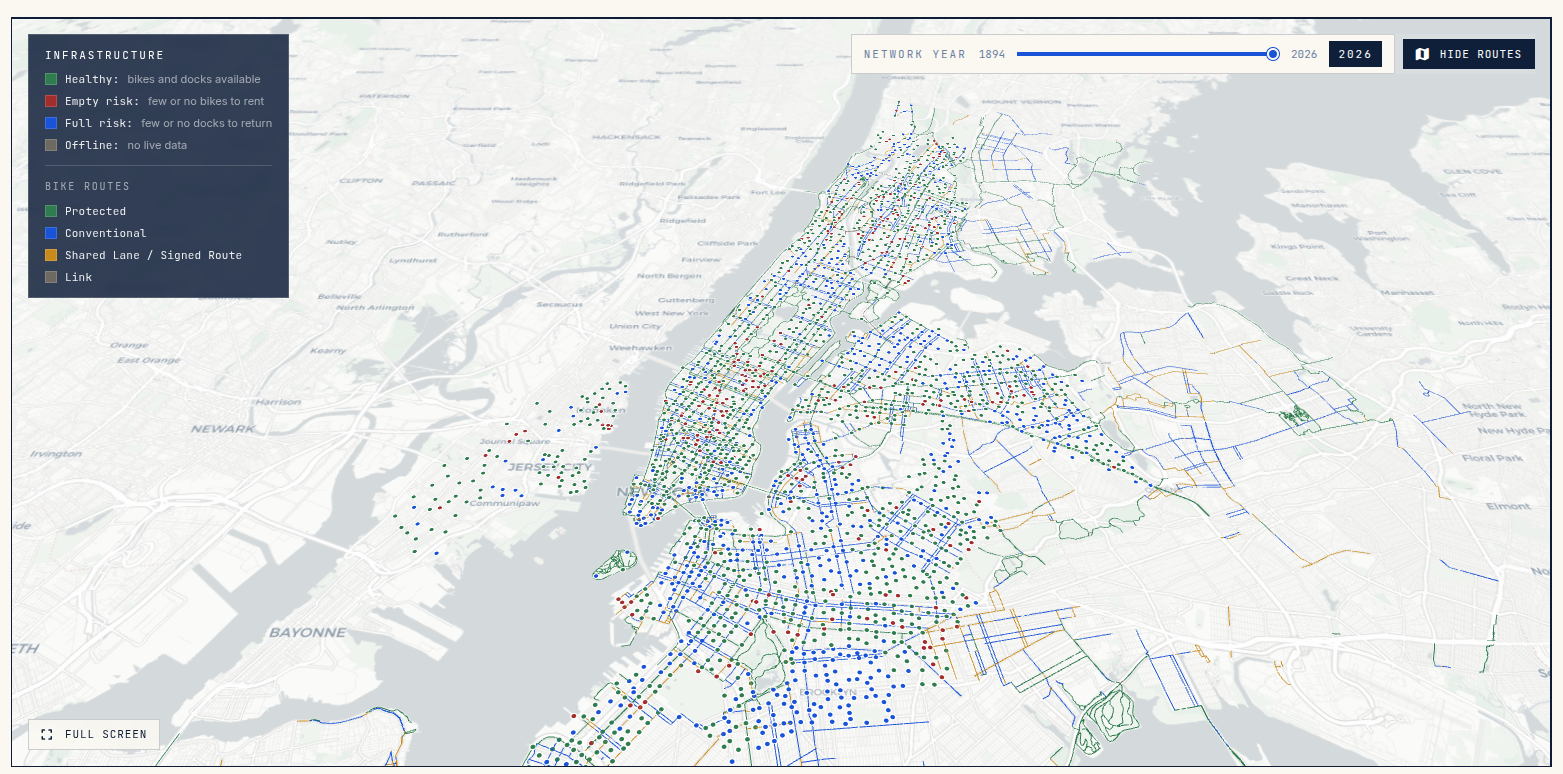
\includegraphics[width=\textwidth]{../media/report/primary_infrastructure_2.png}
        \caption{Infrastructure: the bike routes overlay.}
        \label{fig:viz-infrastructure-bike-routes}
    \end{minipage}
\end{figure}

\begin{figure}[htbp]
    \centering
    \begin{minipage}[t]{0.49\textwidth}
        \centering
        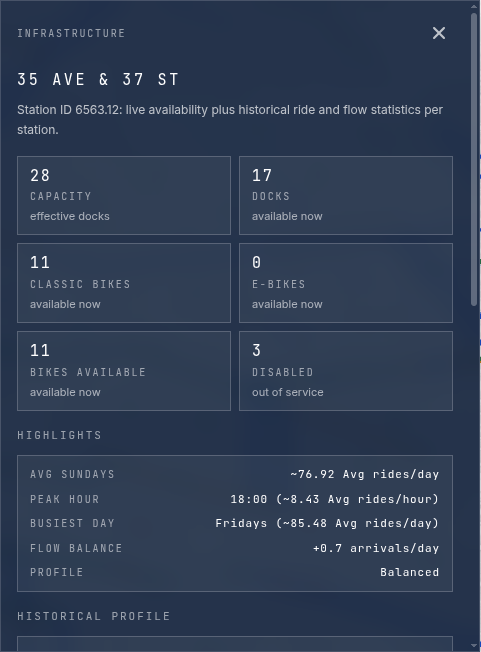
\includegraphics[width=\textwidth]{../media/report/station_sidebar_1.png}
    \end{minipage}
    \hfill
    \begin{minipage}[t]{0.49\textwidth}
        \centering
        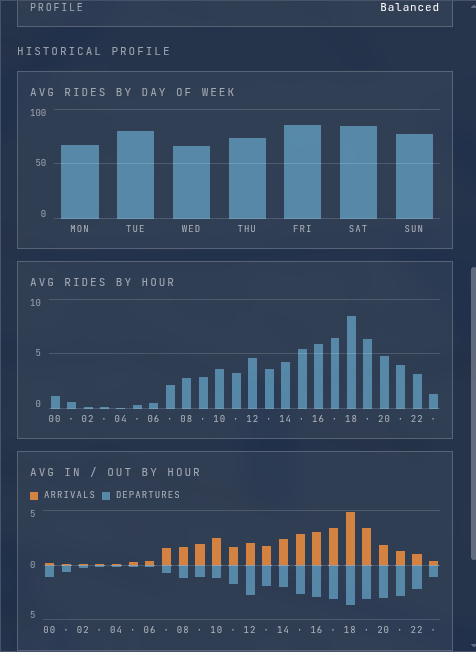
\includegraphics[width=\textwidth]{../media/report/station_sidebar_2.png}
    \end{minipage}
    \caption{Infrastructure: the station sidebar.}
    \label{fig:viz-station-sidebar}
\end{figure}

\paragraph{Network Composition Charts}
Three supplementary plots extend the bike lane infrastructure view (Figure~\ref{fig:viz-secondary-infrastructure}):
\begin{itemize}
    \item \textbf{Network Changes by Year:} A diverging bar chart counting segments installed above the axis and retired below it, giving the temporal overview the map alone cannot convey.
    \item \textbf{Segments by Borough:} A ranked breakdown comparing network size across the five boroughs.
    \item \textbf{Segments by Facility Class:} The same count split by protection level, showing how much of the network is physically separated.
\end{itemize}

\begin{figure}[htbp]
    \centering
    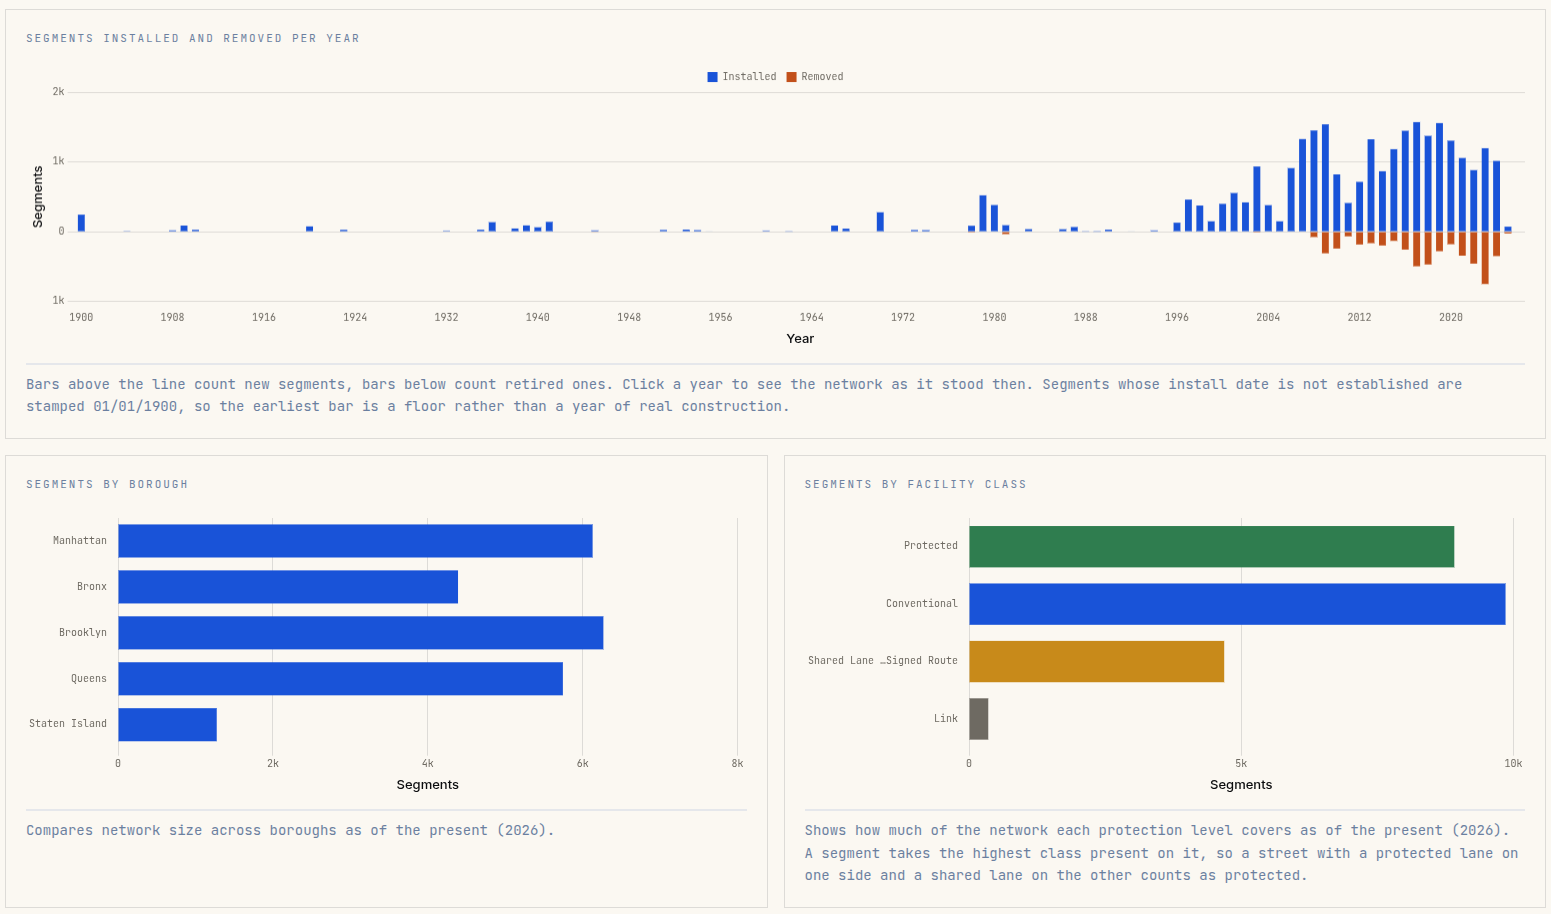
\includegraphics[width=\textwidth]{../media/report/secondary_infrastructure.png}
    \caption{Infrastructure: the supplemental plots.}
    \label{fig:viz-secondary-infrastructure}
\end{figure}

\subsection{Temporal}\label{sec:viz-temporal}
Setting geography aside, this view asks when the system is used.

\paragraph{Surface Graph}
The temporal view features a 3D surface plot mapping activity across days of the week and hours of the day.
Users can switch the metric between average trip volume, duration, distance, and speed.
Furthermore, the plot can be freely rotated to inspect trends from any angle, and hovering over any point reveals exact values (Figure~\ref{fig:viz-temporal-surface}).
This visualization was considered the main view, as its peaks instantly reveal major activity trends at a glance.

\paragraph{Comparison Mode}
Although global filters isolate specific user or bike types, constantly switching between them imposes a heavy cognitive load, as users must memorize the previous view to compare it with the current one.
To address this, we expanded our initial proposal by adding a multi-surface comparison view.
Overlaying surfaces in the same space (Figure~\ref{fig:viz-temporal-compare}) allows direct comparison. 
To prevent overlapping layers from obscuring each other, each surface uses a distinct color scheme with semi-transparent top layers.

To prevent ambiguities, comparison mode enforces three key structural safeguards:
\begin{itemize}
    \item \textbf{Duplicate Prevention:} Prohibits adding duplicate layers, as identical surfaces would only occlude each other without adding analytical value.
    \item \textbf{Filter Consistency:} Clears all pinned comparison layers whenever global header filters change, ensuring stale data is not compared against a newly selected population.
    \item \textbf{Canvas Persistence:} Prevents the removal or hiding of the final active surface so the visual canvas is never left empty.
\end{itemize}

\begin{figure}[htbp]
    \centering
    \begin{minipage}[t]{0.49\textwidth}
        \centering
        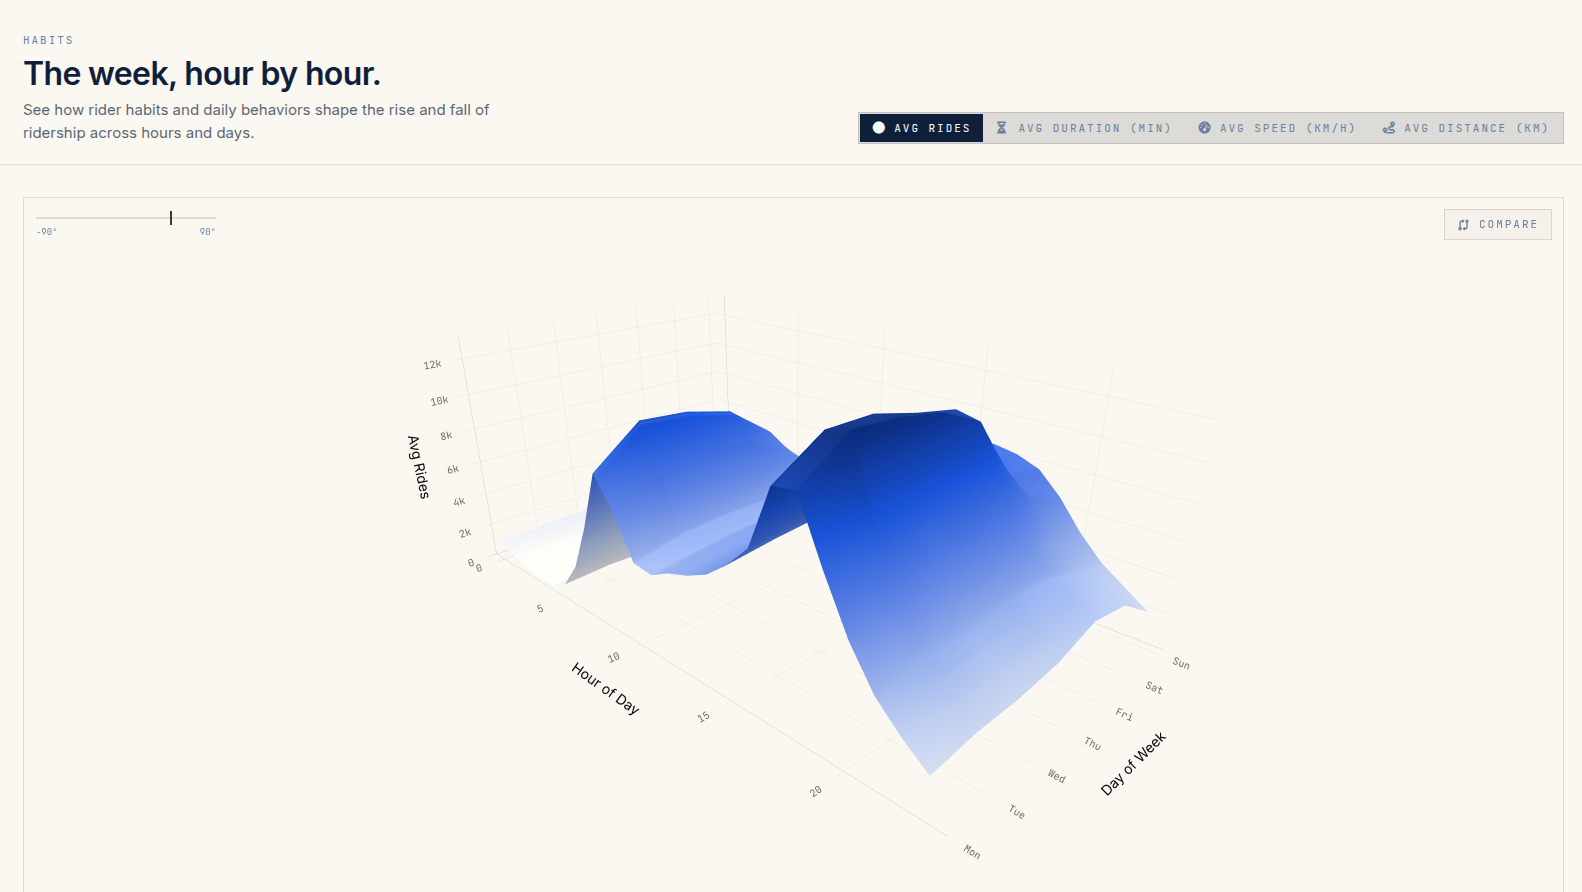
\includegraphics[width=\textwidth]{../media/report/primary_temporal_1.png}
        \caption{Temporal: the day-hour surface.}
        \label{fig:viz-temporal-surface}
    \end{minipage}
    \hfill
    \begin{minipage}[t]{0.49\textwidth}
        \centering
        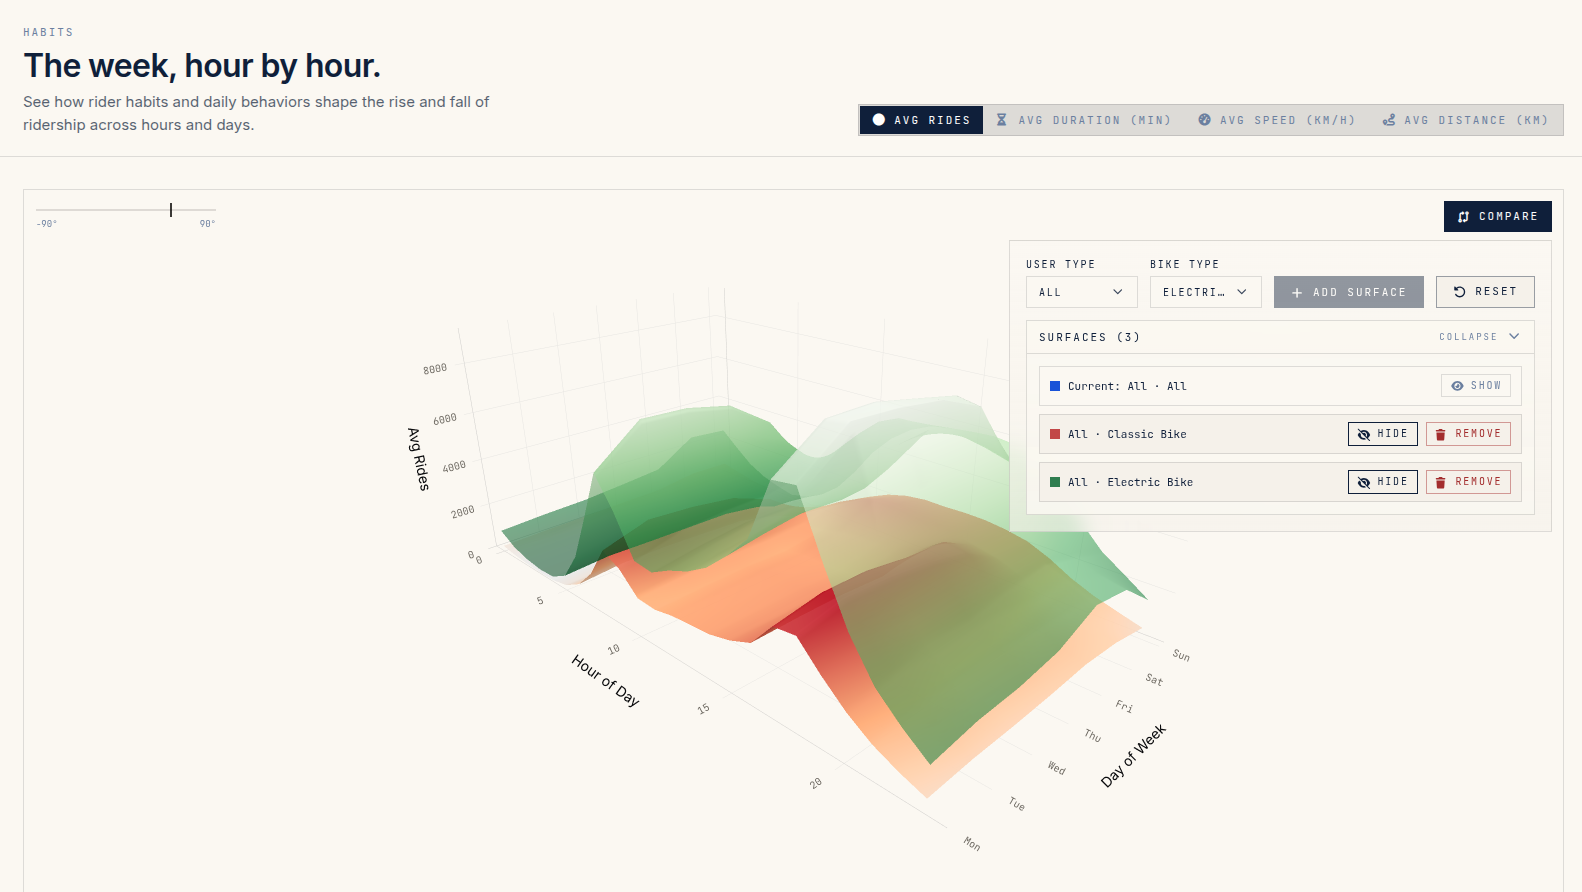
\includegraphics[width=\textwidth]{../media/report/primary_temporal_2.png}
        \caption{Temporal: the comparison mode.}
        \label{fig:viz-temporal-compare}
    \end{minipage}
\end{figure}

\paragraph{Histograms}
The 3D surface plot shows overall shape well, but it makes the detailed distribution of the data hard to see.
To address this, two marginal histograms aggregate data by weekday or hour (Figure~\ref{fig:viz-temporal-hist}).

To make the relationship between the surface and histograms clear, all three views are interactively linked. 
Hovering over a surface cell highlights its corresponding histogram bars, while clicking a bar pins that day or hour. 
Pinned selections project their distribution onto the opposite histogram and overlay a trace line across the 3D surface. 
In comparison mode, the histogram bars match the colors of each active surface (Figure~\ref{fig:viz-temporal-hist-compare}).

\paragraph{Line Chart}
Extreme weather events, like heavy storms, highlighted a gap in our initial design.
Because aggregated charts smooth out this kind of outlier, single-day peaks from weather or holidays were easily missed.
To fix this, we introduced a dedicated line chart plotting every date individually.
This allows us to instantly spot daily outliers, cross-reference data with real-world events, and perform accurate root-cause analysis without losing broader context.

\begin{figure}[htbp]
    \centering
    \begin{minipage}[t]{0.49\textwidth}
        \centering
        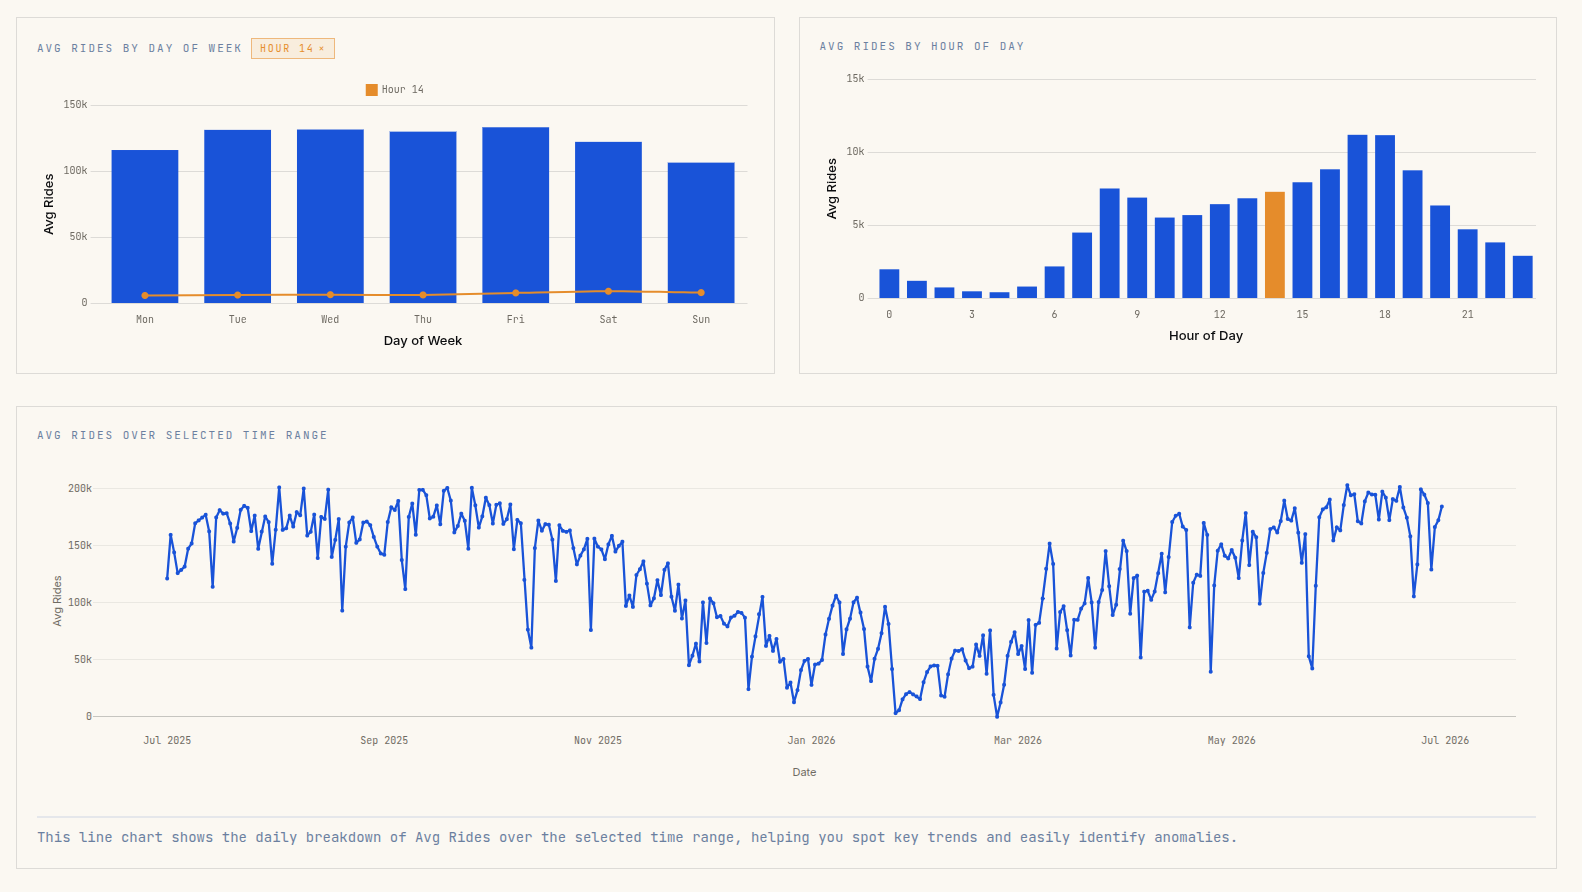
\includegraphics[width=\textwidth]{../media/report/secondary_temporal_1.png}
        \caption{Temporal: the supplemental plots.}
        \label{fig:viz-temporal-hist}
    \end{minipage}
    \hfill
    \begin{minipage}[t]{0.49\textwidth}
        \centering
        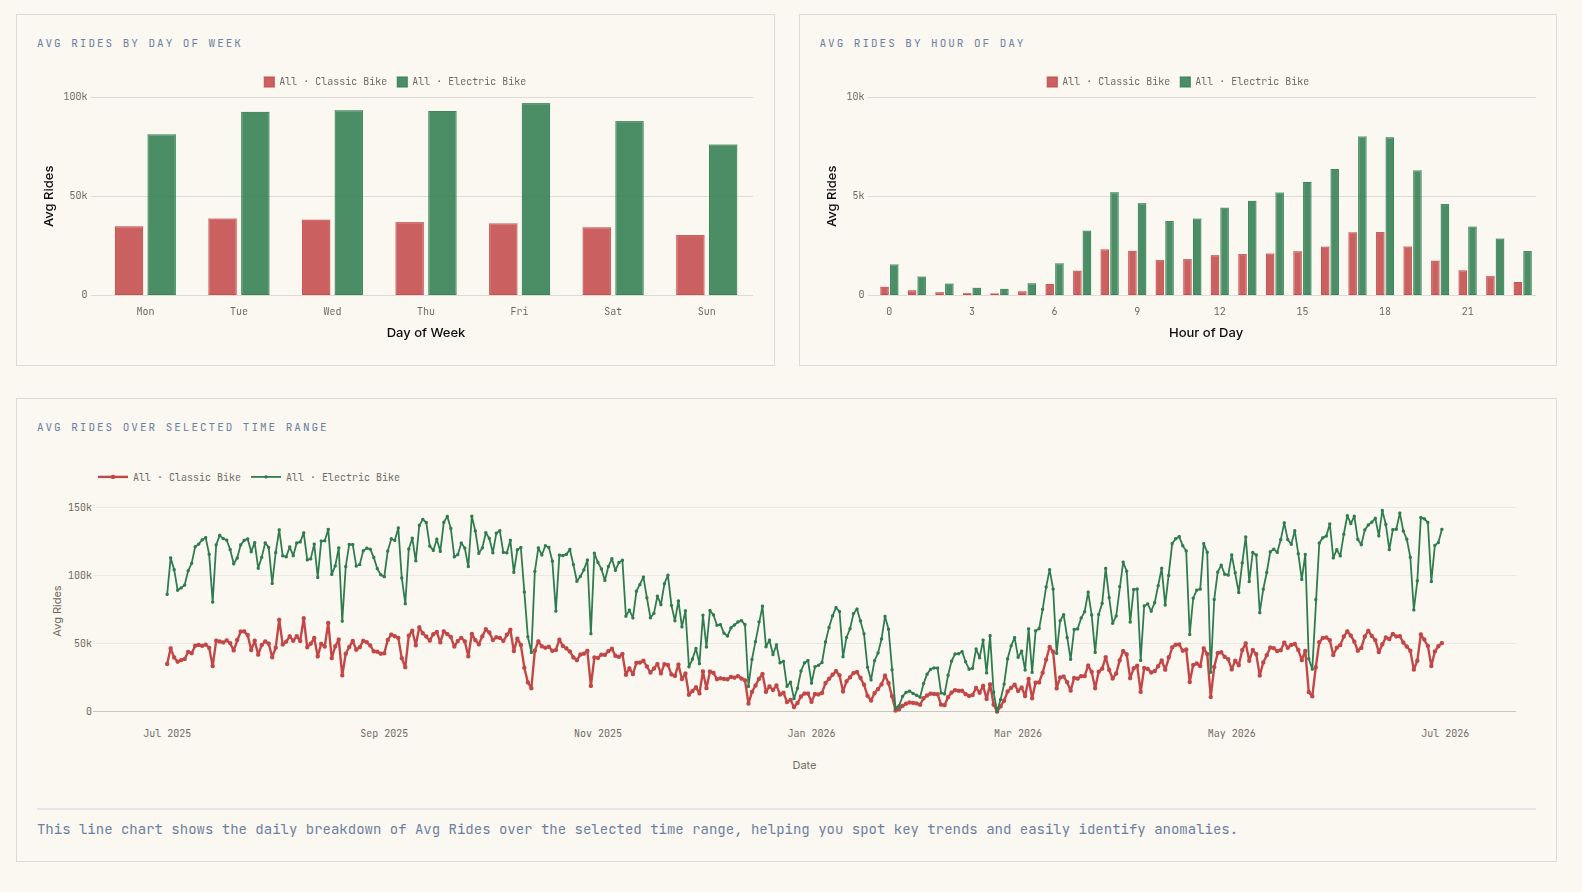
\includegraphics[width=\textwidth]{../media/report/secondary_temporal_2.png}
        \caption{Temporal: the supplemental plots in comparison mode.}
        \label{fig:viz-temporal-hist-compare}
    \end{minipage}
\end{figure}

\subsection{Weather}
This view isolates how much weather changes ridership.

\begin{figure}[htbp]
    \centering
    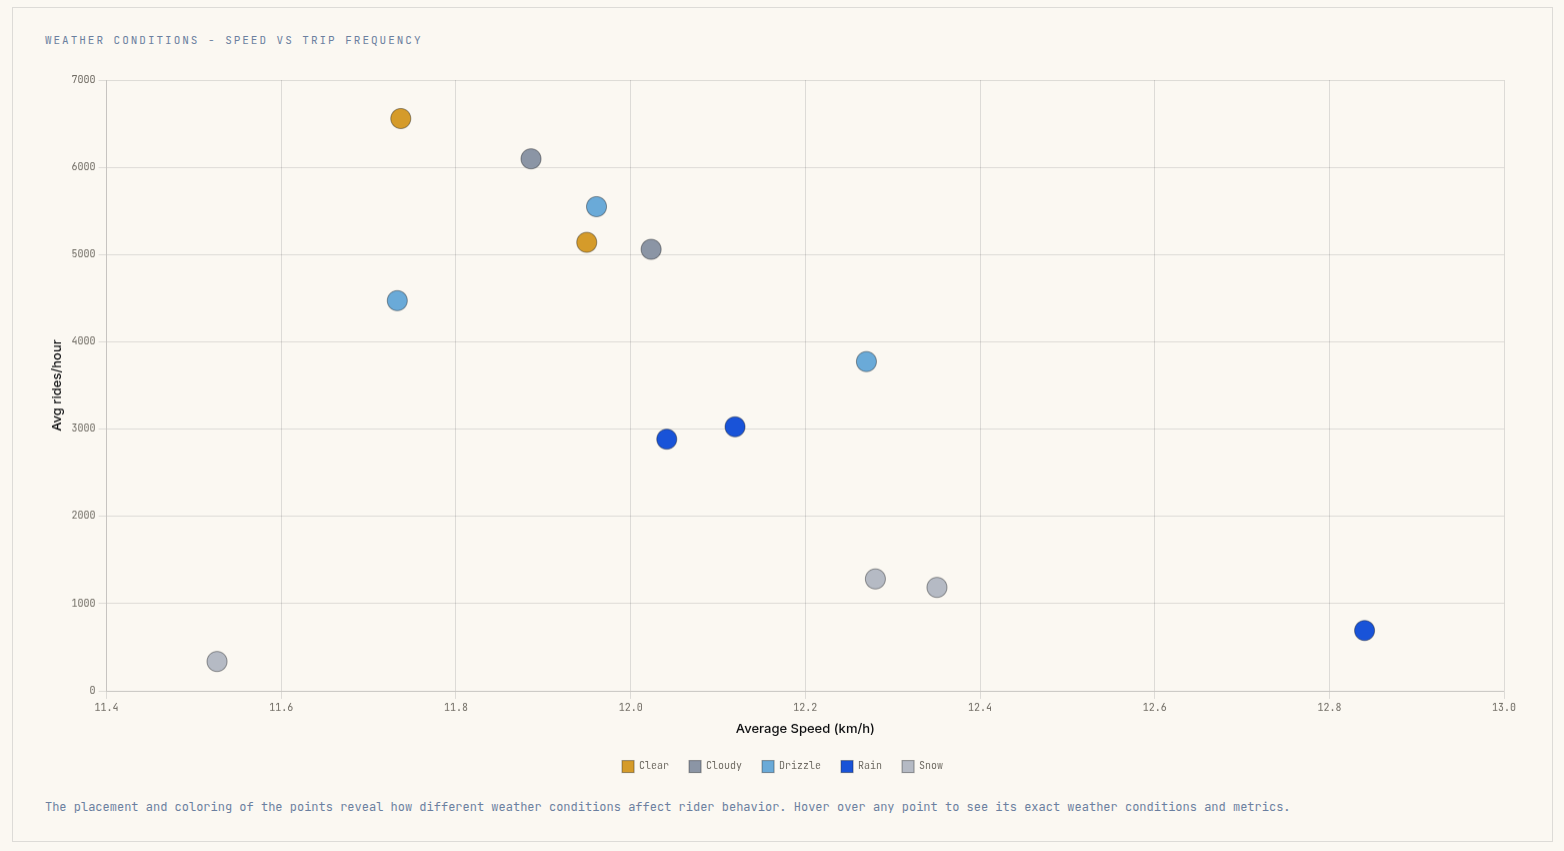
\includegraphics[width=\textwidth]{../media/report/weather_scatterplot.png}
    \caption{Weather: the condition scatter.}
    \label{fig:viz-weather-scatterplot}
\end{figure}

\paragraph{Condition Scatter}
The primary visualization is a scatter plot where each point represents a WMO weather code.
Selecting appropriate axes for the scatter plot required several iterations to make anomalies both visible and explainable.
Initial attempts (such as plotting total rides against temperature) were dominated by common conditions like clear skies, collapsing rare events near the origin.
On the other hand, average duration and average distance increased together in a clear, straight line, rather than forming distinct groups.
Normalizing volume to average hourly rides and pairing it with average trip speed resolved these issues.

Each dot is color-coded by weather condition family (Figure~\ref{fig:viz-weather-scatterplot}), grouping them into high-level categories (e.g., rain, snow, thunderstorm) to simplify interpretation.
This permits intuitive color semantics rather than raw numerical codes, allowing conditions with similar behavioral impacts to form distinct visual clusters.

Then, interactive controls enable deeper data exploration.
Clicking a legend category isolates a specific condition family, while hovering over any data point surfaces a detailed tooltip with weather conditions and trip statistics.
This provides a compact summary of how weather suppresses or sustains global cycling activity.

\paragraph{Ridgeline Distributions}
Although our proposal made the ridgeline chart the primary view, we found it hard to interpret at first glance.
On the other hand, while the scatter plot immediately highlighted key trends, it could not show how usage changed over time.
Rather than removing the ridgeline chart, we moved it to a secondary view to complement the scatter plot.

To capture those missing time shifts, the ridgeline chart plots usage curves for each weather type (Figure~\ref{fig:viz-weather-ridgeline}), complete with an interactive toggle to switch between hourly and weekly views.
During development, we decided to scale each ridge to its own peak.
This design choice made it easy to compare activity patterns between rare events, such as thunderstorms, and baseline clear days.
However, this introduced a key trade-off, as scaling hid absolute ride volumes.
To prevent readers from mistaking relative patterns for total demand, we added clear chart annotations.

\begin{figure}[htbp]
    \centering
    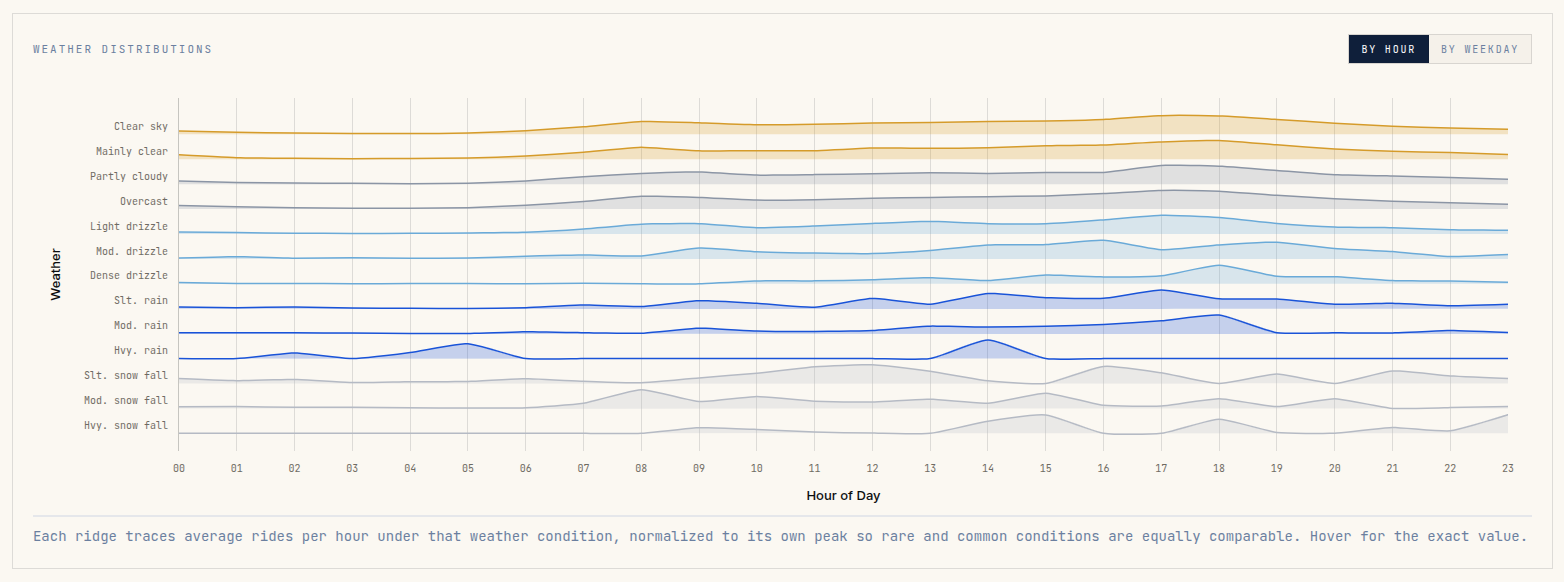
\includegraphics[width=\textwidth]{../media/report/weather_ridgeline.png}
    \caption{Weather: the ridgeline distributions.}
    \label{fig:viz-weather-ridgeline}
\end{figure}

\paragraph{Temperature and Rain Response}
Standard weather categories often group too many days together, hiding crucial details about absolute volume and how temperature or rain specifically affect rider behavior.
To uncover these finer details, two supplementary plots examine continuous weather variables directly (Figure~\ref{fig:viz-secondary-weather}):
\begin{itemize}
    \item \textbf{Temperature Response:} A line chart showing average hourly rides for every one-degree temperature change.
    \item \textbf{Rain Impact:} A bar chart showing the percentage drop in ridership across different rain levels compared to dry weather.
\end{itemize}

\begin{figure}[htbp]
    \centering
    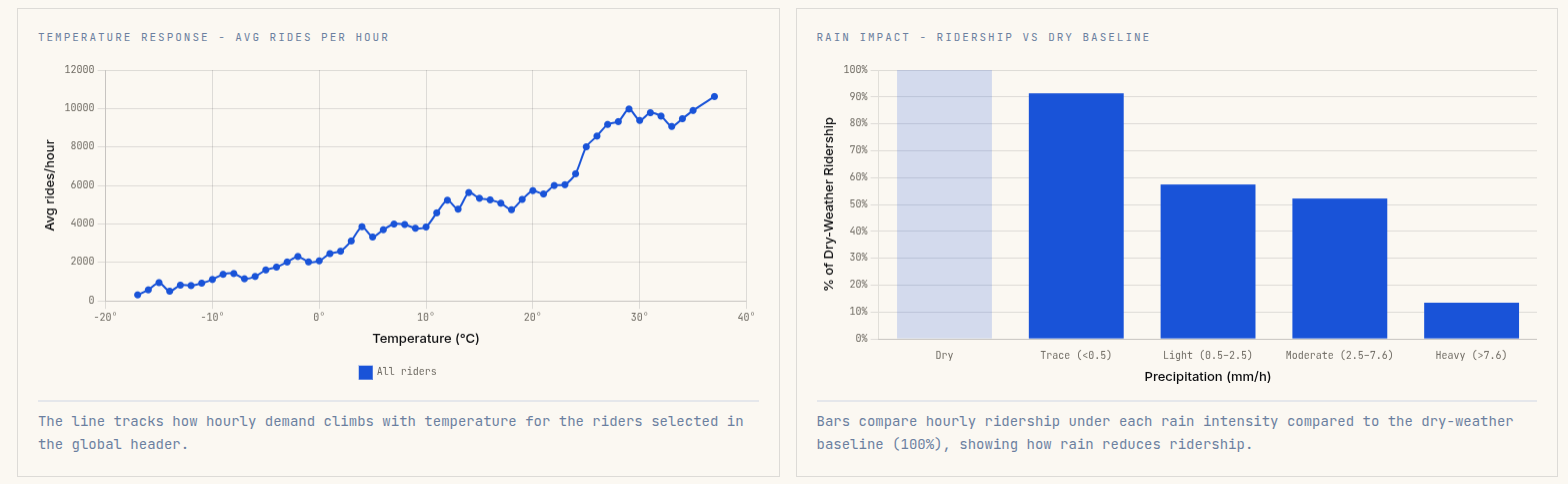
\includegraphics[width=\textwidth]{../media/report/secondary_weather.png}
    \caption{Weather: the supplemental plots.}
    \label{fig:viz-secondary-weather}
\end{figure}

\subsection{Footprint}
The footprint view translates ridden distance into environmental impact using published emission factors.
Because real-world car substitution rates vary significantly across studies and rider demographics, fixing this rate to a single static value would be misleading.
To reflect this real-world uncertainty, an interactive slider allows readers to adjust the substitution rate between $5\%$ and $25\%$, dynamically updating all visualizations to show a range of plausible outcomes.

\paragraph{Tiles and Emission Charts}
Three headline tiles summarize total distance ridden, avoided $\text{CO}_2$, and replaced car trips (Figure~\ref{fig:viz-footprint}).
A horizontal bar chart compares how much emission that same distance produces across transport modes, holding distance constant to highlight efficiency differences.
Finally, a cumulative chart tracks daily avoided $\text{CO}_2$ over time, with a shaded band showing the range between the minimum and maximum substitution rates and a dotted line tracing the user's selected setting.

We chose this dual-layer design to prevent readers from mistaking rough estimates for exact facts.
Showing the full range alongside a moving line lets users explore different assumptions while keeping real-world uncertainty clearly in view.

\begin{figure}[htbp]
    \centering
    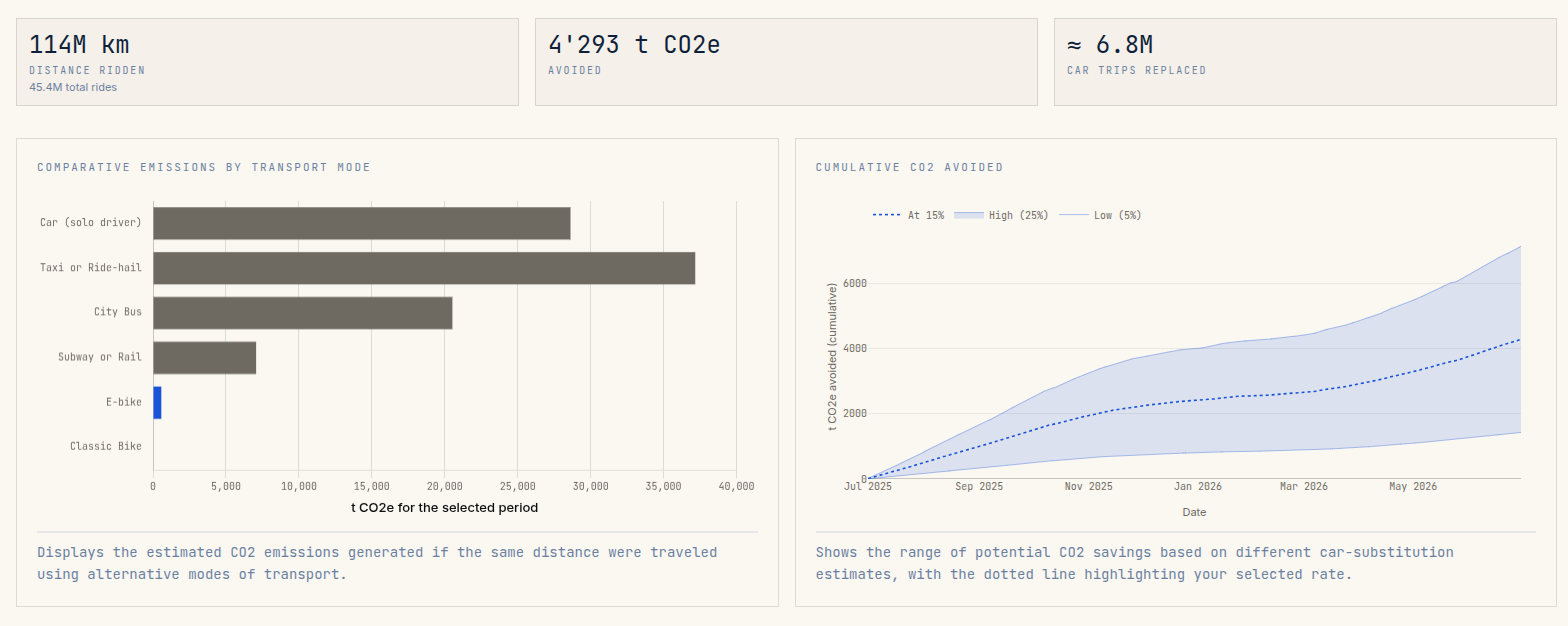
\includegraphics[width=\textwidth]{../media/report/primary_footprint.png}
    \caption{Footprint: the emission tiles and charts.}
    \label{fig:viz-footprint}
\end{figure}

\paragraph{Pictogram}
Because raw carbon tonnage is hard to picture, a pictogram translates these numbers into relatable real-world benchmarks: urban trees absorbing carbon, a person's annual emissions, and powered LED bulbs (Figure~\ref{fig:viz-pictogram}).

To keep the display clean, each row targets roughly $24$ icons by rounding unit values to clean steps (like $1$, $2$, or $5$ times a power of ten).
Adjusting the slider simply changes the number of icons shown. 
However, changing the date range rescales what each icon represents to keep the row length manageable.
\begin{figure}[htbp]
    \centering
    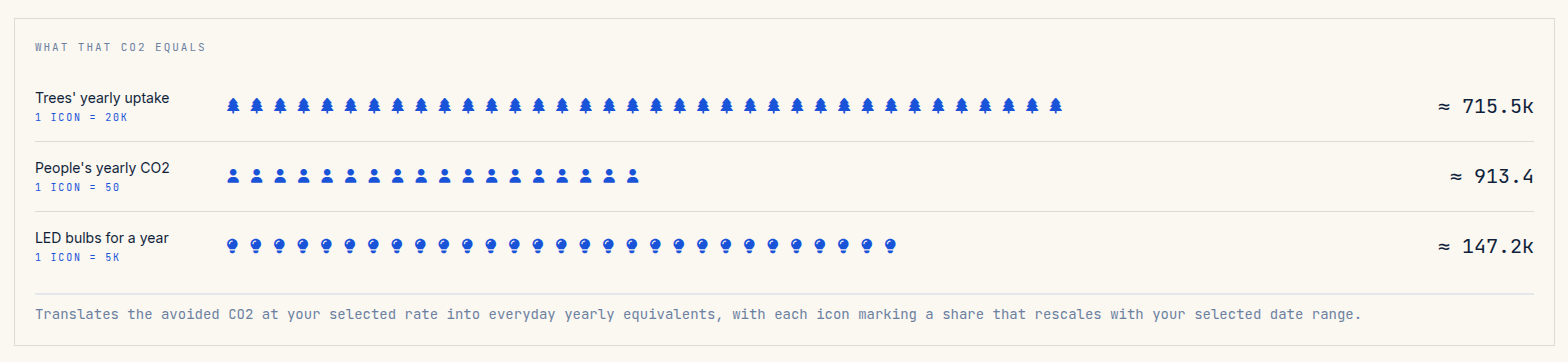
\includegraphics[width=\textwidth]{../media/report/secondary_footprint.png}
    \caption{Footprint: the pictogram.}
    \label{fig:viz-pictogram}
\end{figure}

\paragraph{Assumptions Box}
Unlike other views, this page displays modeled estimates rather than directly measured values.
To prevent users from mistaking avoided $\text{CO}_2$ figures for direct measurements, we prioritized explicit transparency.
An assumptions box outlines all baseline inputs, including transport mode emission factors, substitution rates from cited literature, and computational exclusions (Figure~\ref{fig:viz-assumptions}).
Inline citations provide direct links for verification.

\begin{figure}[htbp]
    \centering
    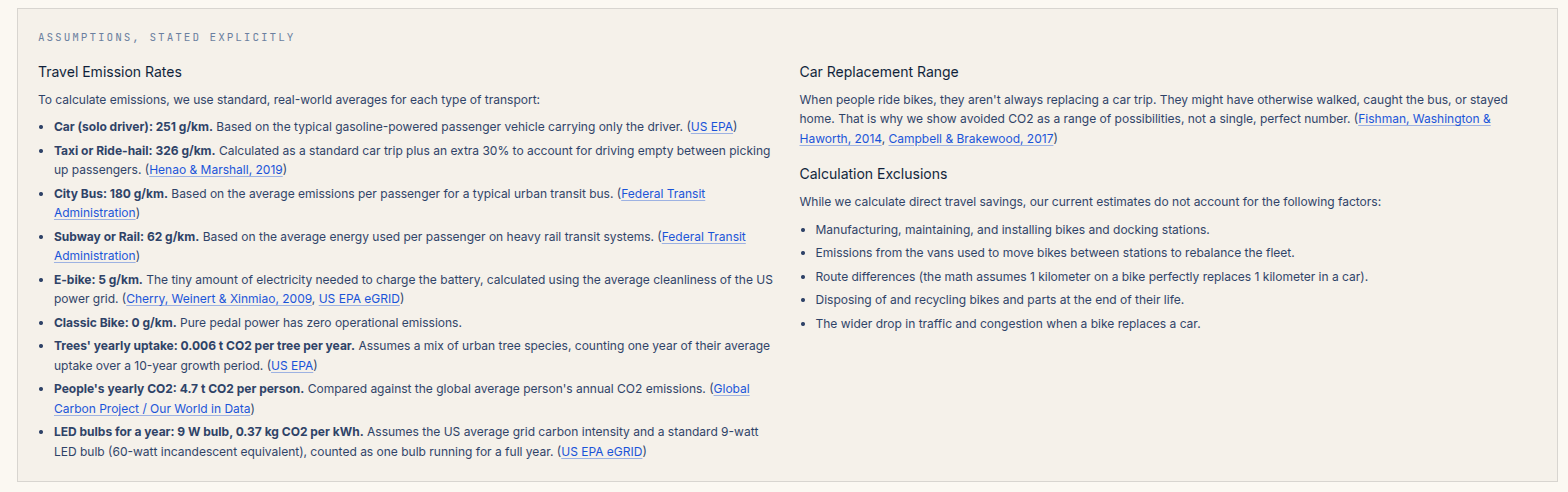
\includegraphics[width=\textwidth]{../media/report/assumption_box.png}
    \caption{Footprint: the assumptions box.}
    \label{fig:viz-assumptions}
\end{figure}
